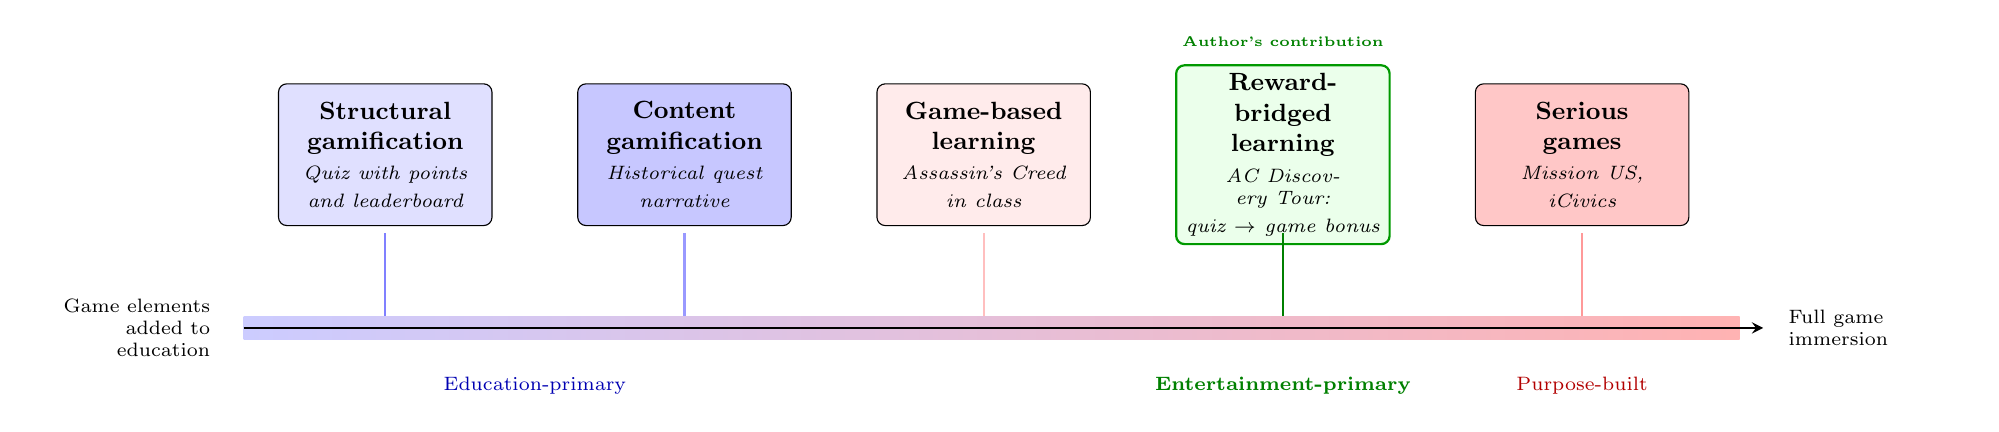
\begin{tikzpicture}[
  every node/.style={font=\small},
  levelbox/.style={rectangle, draw, rounded corners=3pt, minimum width=2.6cm,
    minimum height=1.8cm, text width=2.5cm, align=center, font=\small,
    inner sep=3pt},
  novelbox/.style={rectangle, draw, rounded corners=3pt, minimum width=2.6cm,
    minimum height=1.8cm, text width=2.5cm, align=center, font=\small,
    inner sep=3pt, thick, draw=green!60!black},
]

% Gradient arrow bar
\shade[left color=blue!20, right color=red!30] (0,-0.15) rectangle (19,0.15);
\draw[thick, ->, >=stealth] (0,0) -- (19.3,0);

% Left label
\node[font=\scriptsize, text width=2.2cm, align=right, anchor=east] at (-0.3,0)
  {Game elements\\added to\\education};
% Right label
\node[font=\scriptsize, text width=2.2cm, align=left, anchor=west] at (19.5,0)
  {Full game\\immersion};

% Level 1: Structural gamification
\node[levelbox, fill=blue!12] (L1) at (1.8, 2.2)
  {\textbf{Structural\\gamification}\\[3pt]
   \scriptsize\itshape Quiz with points\\[-1pt]\scriptsize\itshape and leaderboard};
\draw[thick, blue!50] (1.8, 1.2) -- (1.8, 0.15);

% Level 2: Content gamification
\node[levelbox, fill=blue!22] (L2) at (5.6, 2.2)
  {\textbf{Content\\gamification}\\[3pt]
   \scriptsize\itshape Historical quest\\[-1pt]\scriptsize\itshape narrative};
\draw[thick, blue!40] (5.6, 1.2) -- (5.6, 0.15);

% Level 3: Game-based learning
\node[levelbox, fill=red!8] (L3) at (9.4, 2.2)
  {\textbf{Game-based\\learning}\\[3pt]
   \scriptsize\itshape Assassin's Creed\\[-1pt]\scriptsize\itshape in class};
\draw[thick, red!25] (9.4, 1.2) -- (9.4, 0.15);

% Level 4: Reward-bridged learning (NEW — author's contribution)
\node[novelbox, fill=green!8] (L4) at (13.2, 2.2)
  {\textbf{Reward-bridged\\learning}\\[3pt]
   \scriptsize\itshape AC Discovery Tour:\\[-1pt]\scriptsize\itshape quiz $\to$ game bonus};
\draw[thick, green!50!black] (13.2, 1.2) -- (13.2, 0.15);

% Level 5: Serious games
\node[levelbox, fill=red!22] (L5) at (17.0, 2.2)
  {\textbf{Serious\\games}\\[3pt]
   \scriptsize\itshape Mission US,\\[-1pt]\scriptsize\itshape iCivics};
\draw[thick, red!40] (17.0, 1.2) -- (17.0, 0.15);

% Directionality annotation below
\node[font=\scriptsize, blue!70!black, anchor=north] at (3.7, -0.5)
  {Education-primary};
\node[font=\scriptsize, green!50!black, anchor=north, font=\scriptsize\bfseries] at (13.2, -0.5)
  {Entertainment-primary};
\node[font=\scriptsize, red!70!black, anchor=north] at (17.0, -0.5)
  {Purpose-built};

% Novel contribution marker
\node[font=\tiny\bfseries, green!50!black, anchor=south] at (13.2, 3.45)
  {Author's contribution};

\end{tikzpicture}
